\documentclass[fleqn]{jsarticle}
\usepackage{amsmath,amssymb}
\usepackage{fancybox}
\usepackage{ascmac}
\usepackage[dvipdfmx]{graphicx}
\usepackage[dvipdfmx]{hyperref}
\usepackage{pxjahyper}

\begin{document}
	\textgt{Q2} [長さの差]下の図は三角形ABCにおいて,頂点Aから辺BCの延長へ垂線を下したものです。垂線の足をHとし,BHの長さがlcm,∠BAC=48°,∠C=28°のとき,辺の長さの差AC—BCの大きさはいくらですか。\\
	\begin{figure}[h]
		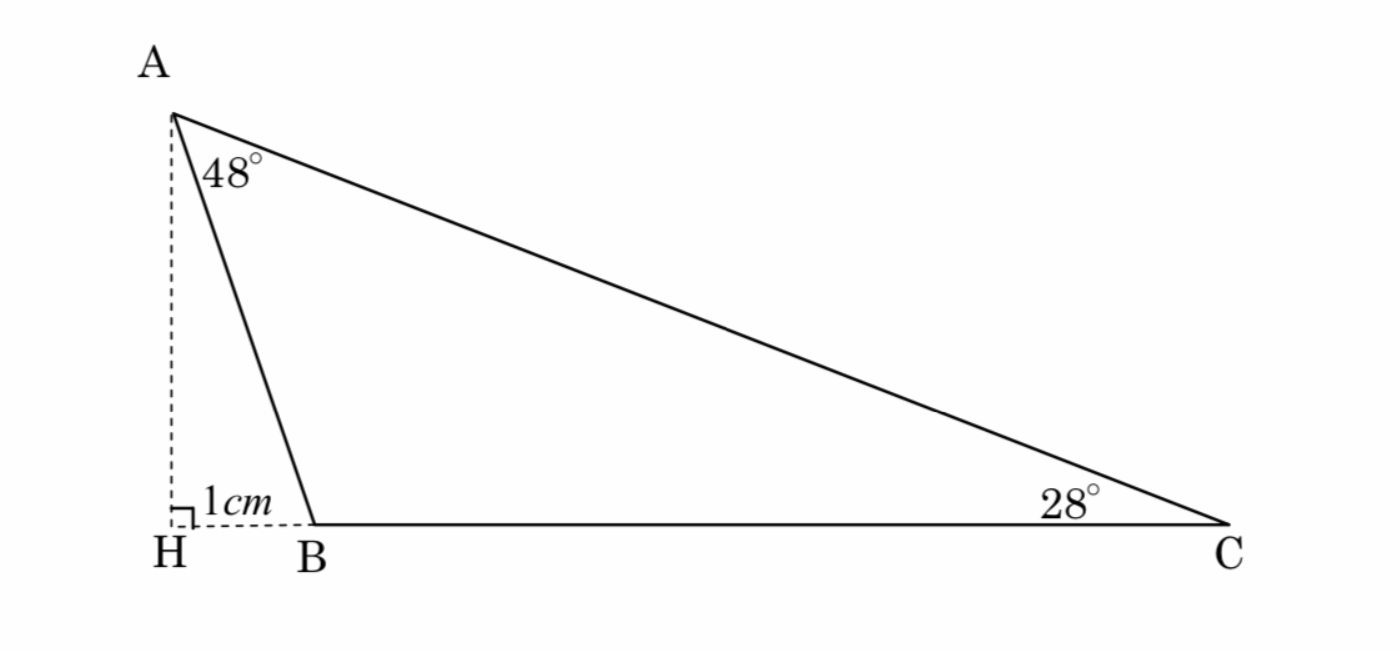
\includegraphics[width=14.0cm]{./2020-05-05-092534.png}
	\end{figure}
	\\
	\ovalbox{解答}\\
	\begin{figure}[h]
		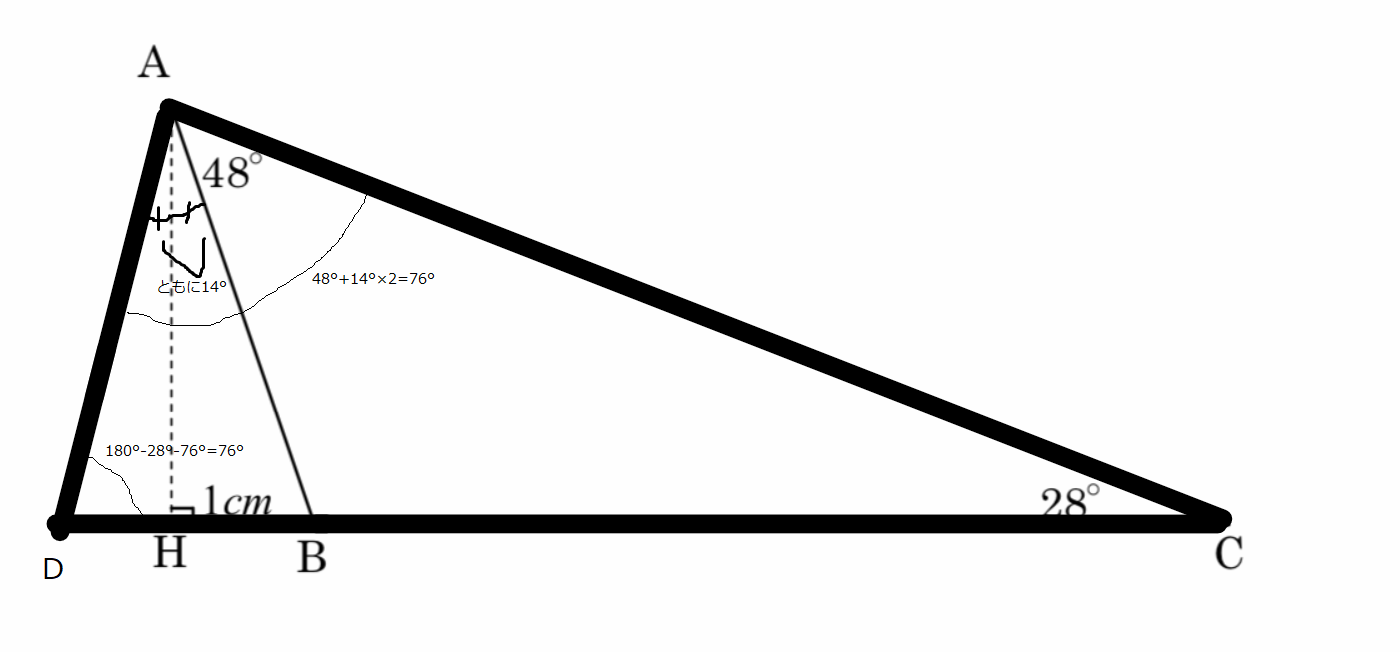
\includegraphics[width=14.0cm]{./2020-05-05-092534ed.png}
	\end{figure}
	\\
	$\angle{BCA}$の大きさは、$28°$で、$\angle{AHC}$の大きさは$90°$あるから、$\angle{CAH}$の大きさは、\\
	$\angle{CAH}=180°-28°-90°=62°$\\
	したがって、$\angle{HAB}$=$62°-48°$=$14°$\\
	となる。ここで、線分CBの延長線上に、$\angle{DAH}$=$14°$となるようなDをとる。\\
	このとき、$\angle{CAD}=\angle{CAH}+\angle{DAH}=62°+14°=76°$\\
	また$\angle{CDA}=180°-28°-76°=76°$\\
	したがって、$\angle{CAD}=\angle{CDA}$となり、$\triangle{CAD}$は二等辺三角形になる。\\
	したがって、$CA=CD$\\
	また、$\angle{BAH}=\angle{DAH}、AH⊥BDより、BH=DH$であるから、$BD=1\times 2=2$\\
	$AC-BC=CA-BC=CD-CB=2$cm\\
	\\
	\vspace{5cm}
	\\
	※実際にはぜんぜんおもいつかなくて、三角関数つかって解いてしまった(´・ω・`)\\
	\\
	$\frac{1}{\sin 14^\circ}=\frac{AB}{\sin 90^\circ}$\\
	$\therefore AB=\frac{\sin 90^\circ}{\sin 14^\circ}$\\
	また$\frac{AB}{\sin 28^\circ}=\frac{AC}{\sin (180^\circ-48^\circ-28^\circ)}=\frac{BC}{\sin 48^\circ}$より\\
	$AC=\frac{\sin 104^\circ}{\sin 28^\circ}AB$\\
	$BC=\frac{\sin 48^\circ}{\sin 28^\circ}AB$\\
	$\therefore AC=\frac{\sin 104^\circ \sin 90^\circ}{\sin 28^\circ \sin 14^\circ}$\\
	$BC=\frac{\sin 48^\circ \sin 90^\circ}{\sin 28^\circ \sin 14^\circ}$\\
	$\therefore AC-BC=\frac{\sin 104^\circ \sin 90^\circ}{\sin 28^\circ \sin 14^\circ}-\frac{\sin 48^\circ \sin 90^\circ}{\sin 28^\circ \sin 14^\circ}$\\
	\begin{figure}[h]
		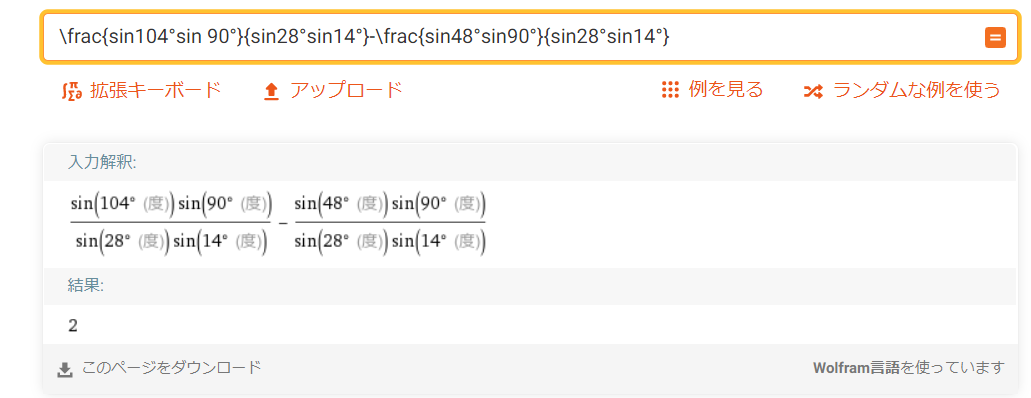
\includegraphics[width=14cm]{./2020-05-05-102216.png}
	\end{figure}\\
	\href{https://www.wolframalpha.com/input/?i=\%5Cfrac\%7Bsin104\%C2\%B0sin+90\%C2\%B0\%7D\%7Bsin28\%C2\%B0sin14\%C2\%B0\%7D-\%5Cfrac\%7Bsin48\%C2\%B0sin90\%C2\%B0\%7D\%7Bsin28\%C2\%B0sin14\%C2\%B0\%7D\&lang=ja}{https://www.wolframalpha.com/input/?i=\%5Cfrac\%7Bsin104\%C2\%B0sin+90\%C2\%B0\%7D\%7Bsin28\%C2\%B0sin14\%C2\%B0\%7D-\%5Cfrac\%7Bsin48\%C2\%B0sin90\%C2\%B0\%7D\%7Bsin28\%C2\%B0sin14\%C2\%B0\%7D\&lang=ja}
\end{document}